%
% Modelo de artigo científico em português brasileiro e em conformidade com as normas da ABNT
% Documento principal
%
% *****************************************************************************
% *  Centro Federal de Educação Tecnológica de Minas Gerais - CEFET-MG        *
% *  Laboratório de Sistemas Inteligentes - LSI                               *
% *                                                                           *
% *  Autor: Denise de Souza <densouza@gmail.com>                              *
% *  Autor: Henrique E. Borges <henrique@lsi.cefetmg.br>                      *
% *                                                                           *
% *****************************************************************************



\documentclass[
%   opções da classe memoir
      article,					% Indica que é um artigo científico
      %11pt,					% Tamanho da fonte
      twocolumn,				% Número de colunas
      %twoside,					% Impressão em frente (anverso) e verso. Oposto a oneside
      %oneside,					% Impressão apenas no anverso. Oposto a twoside
      a4paper,					% Tamanho do papel
%   opções da classe abntex2
      %chapter=TITLE,			% Títulos de capítulos convertidos para letras maiúsculas
      %section=TITLE,			% Títulos de seções convertidos para letras maiúsculas
      %subsection=TITLE,		% Títulos de subseções convertidos para letras maiúsculas
      %subsubsection=TITLE 		% Títulos de subsubseções convertidos para letras maiúsculas
%   opções do pacote babel
      english,					% Idioma adicional para hifenização
      brazil,					% O ultimo idioma indicado será o principal idioma do documento
      sumario=tradicional
]{abntex2} 



% -----------------------------------------------------------------------------
%    Pacotes fundamentais 
% -----------------------------------------------------------------------------

\usepackage[T1]{fontenc}		% Seleção de código de fonte
\usepackage{lmodern}			% Usa a fonte Latin Modern
%\usepackage[latin1]{inputenc}	% Codificação do documento (conversão automatica dos acentos)
\usepackage[utf8]{inputenc}		% Codificação do documento (conversão automatica dos acentos)
\usepackage{indentfirst}		% Indenta o primeiro parágrafo de cada seção.
\usepackage{nomencl} 			% Lista de símbolos
\usepackage{color}				% Controle das cores
\usepackage{graphicx}			% Inclusão de gráficos
\usepackage{microtype} 			% Melhora a justificação do documento
\usepackage{comandos} 			% Novos comandos
\usepackage{tikz}	 			% Pacote para desenhos
\usepackage{etoolbox}	 		% Pacote para tratamento de condicionais (if-else-end \ string)
\usepackage{ifthen}				% Pacote para tratamento de condicionais (if-else-end \ number)
\usepackage{balance}			% Balanceia o texto no artigo
\usepackage{babel}				% Usado para definir idioma do documento e respectivas hifenizações



% -----------------------------------------------------------------------------
%    Configura as citações
% -----------------------------------------------------------------------------

\usepackage[alf]{abntex2cite}		% Formata as citações bibliográficas conforme a norma ABNT
%\usepackage[alf, 					% Formata as citações bibliográficas conforme a norma ABNT
%	abnt-emphasize=bf, 
%	bibjustif, 
%	recuo=0cm, 
%	abnt-etal-cite=2, 
%	abnt-etal-list=0]{abntex2cite}


% -----------------------------------------------------------------------------
%   Configurações de aparência do PDF final
% -----------------------------------------------------------------------------

\definecolor{blue}{RGB}{41,5,195}	% Altera o aspecto da cor azul

\makeatletter
\hypersetup{
  %pagebackref=true,
  %pdftitle={\@title}, 
  %pdfauthor={\@author},
  %pdfsubject={Modelo de artigo científico com abnTeX2},
  %pdfcreator={LaTeX with abnTeX2},
  %pdfkeywords={abnt}{latex}{abntex}{abntex2}{artigo científico}, 
  colorlinks=true,       	% true: “links” coloridos; false: “links” em caixas de texto
  linkcolor=blue,			% Define cor dos “links” internos”
  citecolor=blue,			% Define cor dos “links” para as referências bibliográficas
  filecolor=magenta,		% Define cor dos “links” para arquivos
  urlcolor=blue,			% Define a cor dos “hiperlinks”
  bookmarksdepth=4
}
\makeatother



% -----------------------------------------------------------------------------
%   Compila o índice
% -----------------------------------------------------------------------------

\makeindex



% -----------------------------------------------------------------------------
%   Configurações do modelo de artigo em inglês
% -----------------------------------------------------------------------------

\usepackage[hmarginratio=1:1,top=32mm,columnsep=20pt]{geometry}		% Formata as margens do artigo
\usepackage{multicol} 				% Usado para “layout” do documento em duas-colunas

\usepackage[hang, small,labelfont=bf,up,textfont=it,up]{caption} 	% Formata as legendas inferiors/superiores em ilustrações (tabelas/figuras)
\usepackage{booktabs} 				% Réguas horizontais em tabelas
\usepackage{float} 					% Necessário para tabelas/figuras em ambiente multi-colunas
									% Devem ser, necessariamente, colocados em pontos específicos junto com [H] (e.g., \begin{table}[H])
\usepackage{hyperref} 				% Usado para criar “hyperlinks” no PDF

%\usepackage{lettrine} 				% Lettrine é a primeira letra do início de um texto que é aumentada em relação às demais

\usepackage{paralist} 				% Usado para diminuir o espaçamento entrelinhas em listas de “bullets”

\usepackage{abstract} 				% Possibilita a customização do “Abstract”
\renewcommand{\abstractnamefont}{\normalfont\bfseries} 		% Define a palavra "Abstract" como negrito e tamanho normal
\renewcommand{\abstracttextfont}{\normalfont\small\itshape} % Define o conteúdo de “Abstract” como itálico e tamanho pequeno

\usepackage{titlesec} 				% Possibilita a customização dos títulos das seções
% \renewcommand\thechapter{\Roman{chapter}}		 	% Capítulos numerados com algarismos romanos
% \renewcommand\thesection{\Roman{section}} 		% Seções numeradas com algarismos romanos
% \renewcommand\thesubsection{\Roman{subsection}} 	% Subseções numeradas com algarismos romanos
\titleformat{\chapter}[block]{\vspace{-0.5cm}\large\scshape\centering\vspace{-0.5cm}}{}{0em}{} 					% Formata os títulos dos capítulos
\titleformat{\section}[block]{\large\scshape\centering}{\thesection\hspace{0.5em}--\hspace{0.5em}}{0em}{}  		% Formata os títulos das seções
\titleformat{\subsection}[block]{\large}{\thesubsection\hspace{0.5em}--\hspace{0.5em}}{0em}{} 					% Formata os títulos das subseções
% \titleformat{\section}[block]{\large\scshape\centering}{\thesection.}{1em}{} 	% Formata os títulos das seções
% \titleformat{\subsection}[block]{\large}{\thesubsection.}{1em}{} 				% Formata os títulos das subseções

\let\footruleskip\undefined
\usepackage{fancyhdr}			  % Possibilita a customização de cabeçalhos e rodapés
\pagestyle{fancy} 				  % Todas as páginas tem cabeçalho e rodapé
\fancyhead{} 					  % Cabeçalho padrão em branco
\fancyfoot{}					  % Rodapé padrão em branco
\fancyhead[C]{\hspace{0.5cm}\imprimirTitulo}	% Customiza o texto do cabeçalho
\fancyfoot[C]{\thepage} 						% Customiza o texto do rodapé



% -----------------------------------------------------------------------------
%   Configura o artigo científico
% -----------------------------------------------------------------------------

\begin{document}

%\maketitle 				  % Insere título (modificado via pacote "comandos")
\pagestyle{fancy} 		      % Todas as páginas tem cabeçalho e rodapé
\thispagestyle{fancy} 		  % Todas as páginas tem cabeçalho e rodapé


%   Insere elementos pré-textuais

% -----------------------------------------------------------------------------
%   Arquivo: ./01-texto/dadosArtigo.tex
% -----------------------------------------------------------------------------


% -----------------------------------------------------------------------------
%   Edite a variável abaixo: substitua "Meu título" pelo título real do artigo
% -----------------------------------------------------------------------------

\tituloA{Trabalho Final de Laboratório de Inteligência Artifical: Localização de Prestadores de Serviços em Redes Sociais Utilizando Busca em Profundidade Limitada}



% -----------------------------------------------------------------------------
%   Edite a variável abaixo: indicando os nomes do autor principal e de até 4 co-autores.
%   Não havendo co-autores, ou se houver menos que 3 deles, deixe os campos entre colchetes em branco (e.g., {})
% -----------------------------------------------------------------------------

\autoresA{Diego Ascânio Santos}{Matheus Ibrahim Nesteruk Moreira}{Ana Carolina Guimarães}{}



% -----------------------------------------------------------------------------
%   Edite a variável abaixo: indicando os nomes das instituições de afiliação tanto do autor principal quanto de até 3 co-autores.
%   Não havendo co-autores, ou se houver menos que 4 deles, deixe os respectivos campos entre colchetes em branco (e.g., {})
% -----------------------------------------------------------------------------

\filiacaoA{Centro Federal de Educação Tecnológica de Minas Gerais}{Centro Federal de Educação Tecnológica de Minas Gerais}{Centro Federal de Educação Tecnológica de Minas Gerais}{}



% -----------------------------------------------------------------------------
%   Edite a variável abaixo: indicando o nome do autor correspondente (aquele que submeteu o artigo) e seu e-mail.
%   O autor correspondente deve ser, necessariamente, um dos autores do artigo
% -----------------------------------------------------------------------------

\autorcorrespondente{Diego Ascânio Santos}{diego@contagem.cefetmg.br}
		% Arquivo a ser editado: contém os dados relativos ao artigo científico
% -----------------------------------------------------------------------------
%   Arquivo: ./01-texto/resumo.tex
% -----------------------------------------------------------------------------

\resumoA{
Encontrar prestadores de serviço pode ser uma tarefa árdua. Este trabalho propõe a utilização de redes sociais para facilitar esse processo, selecionando profissionais dentre amigos ou no máximo amigos dos amigos de um usuário, de forma a levar as tradições presentes no mundo real (de pedir indicações de profissionais a amigos e contactar amigos para a realização de serviços, por questões de confiança) para o âmbito das amizades virtuais.
Para encontrar tais prestadores, mapeia-se uma rede social em um grafo e utiliza-se uma busca em profundidade limitada em nível 2 para alcançar os resultados esperados - uma lista de indivíduos que prestam um serviço desejado, onde esses individuos são amigos diretos do usuário ou amigos de amigos do usuário.
}


\palavrachaveA{
Redes Sociais. Grafos. DLS. DFS. Prestadores de Serviço.
}


% -----------------------------------------------------------------------------
%   Escolha de 3 a 6 palavras ou termos que descrevam este trabalho. As palavras-chaves são utilizadas para indexação.
%   A letra inicial de cada palavra deve estar em maiúsculas. As palavras-chave são separadas por ponto.
% -----------------------------------------------------------------------------
			% Arquivo a ser editado: contém o “resumo” em português brasileiro
\imprimirDadosArtigo				% Comando para imprimir os dados do artigo (título, autores e respectivas afiliações


%   Insere elementos textuais

% -----------------------------------------------------------------------------
%   Arquivo: ./01-texto/introducao.tex
% -----------------------------------------------------------------------------



\section{Introdução}\label{sec:introducao}


%\lettrine[nindent=0em,lines=3]{A}		% Aumenta a primeira letra do primeiro parágrafo da seção

A localização de prestadores de serviço de confiança é uma tarefa que muitas vezes demanda uma grande quantidade de tempo, assim como uma boa dose de sorte para encontrar um prestador de qualidade. Nos dias atuais, as redes sociais promoveram uma interligação massiva entre pessoas de diversas partes do mundo e um professor do Centro Federal de Educação Tecnológica - Prof. Dr. Fábio Rocha da Silva viu um potencial de utilização das redes sociais para o encontro de prestadores de serviço, dando essa ideia para seus alunos em sala de aula.

Cursando a disciplina de Inteligência Artificial, o autor deste artigo viu uma técnica de busca em grafos - Busca em Profunidade Limitada (Depth Limited Search), baseada na busca em profundidade DFS, existente no livro de algoritmos de \citeonline{Cormen} que pôde ser utilizada para implementar a ideia proposta.

A implementação do trabalho utilizou a linguagem Python para simular a rede social e implementar a busca em profundidade limitada, assim como a biblioteca vis, desenvolvida em javascript para visualizar a rede social gerada.
		% Arquivo a ser editado: contém a seção de “introdução” do artigo
% -----------------------------------------------------------------------------
%   Arquivo: ./01-texto/desenvolvimento.tex
% -----------------------------------------------------------------------------


\section{Desenvolvimento}\label{sec:desenvolvimento}	% edite para alterar o título da seção

Implementou-se em linguagem python uma abstração de uma rede social, contendo indivíduos e conexões entre os mesmos.

Para isso, criou-se uma classe Individuo (para representar um individuo da rede social), contendo somente dois atributos: id e profissão, ambos do tipo inteiro.

\begin{center}
  \captionof{figure}{Classe Individuo}
  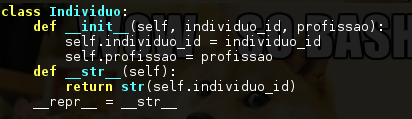
\includegraphics[scale=0.45]{./02-figuras/individuo.png}
  \label{fig:patoA}
\end{center}

Cada individuo tem uma profissão e para esta simulação, foram definidas 5 profissões possíveis:

\begin{center}
  \captionof{figure}{Profissões Possíveis}
  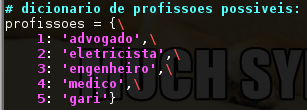
\includegraphics[scale=0.45]{./02-figuras/profissoes.png}
  \label{fig:patoA}
\end{center}


Neste problema, definiu-se que a rede social simulada terá 20 individuos. Para isso, foi criada uma lista de individuos:

\begin{center}
  \captionof{figure}{Lista de Individuos}
  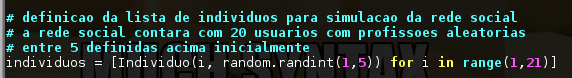
\includegraphics[scale=0.35]{./02-figuras/lista_individuos.png}
  \label{fig:patoA}
\end{center}

A rede social com seus indivíduos e suas amizades foi expressa como um grafo bi direcional e implementada utilizando-se a estrutra de dados dict (dicionário) nativa da linguagem python. Essa estrutura de dados consiste em uma tabela do tipo Chave-Valor, onde ela retorna os valores de uma determinada chave. Um grafo com vários vértices e arestas é bem representado pela estrutura dict, pois seus vértices são as chaves do dicionário e os valores dessas chaves são os vértices adjacentes a ela, representado assim as arestas do grafo.

\begin{center}
  \captionof{figure}{Implementação inicial da Rede Social}
  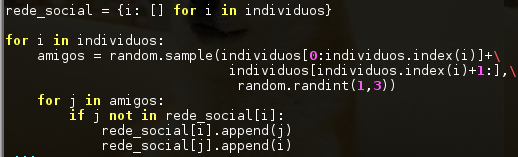
\includegraphics[scale=0.35]{./02-figuras/dict.png}
  \label{fig:patoA}
\end{center}


A primeira abordagem foi a geração aleatória de amizades entre individuos e inserção dessas amizades na rede social. Uma rede aleatória foi gerada e visualizada mediante o auxílio da ferramenta vis. 
A \textbf{Figura \ref{fig:patoB}} representa a visualização gerada.

\begin{figure*}
	\centering
	\caption{Visualização da Rede Social} 
	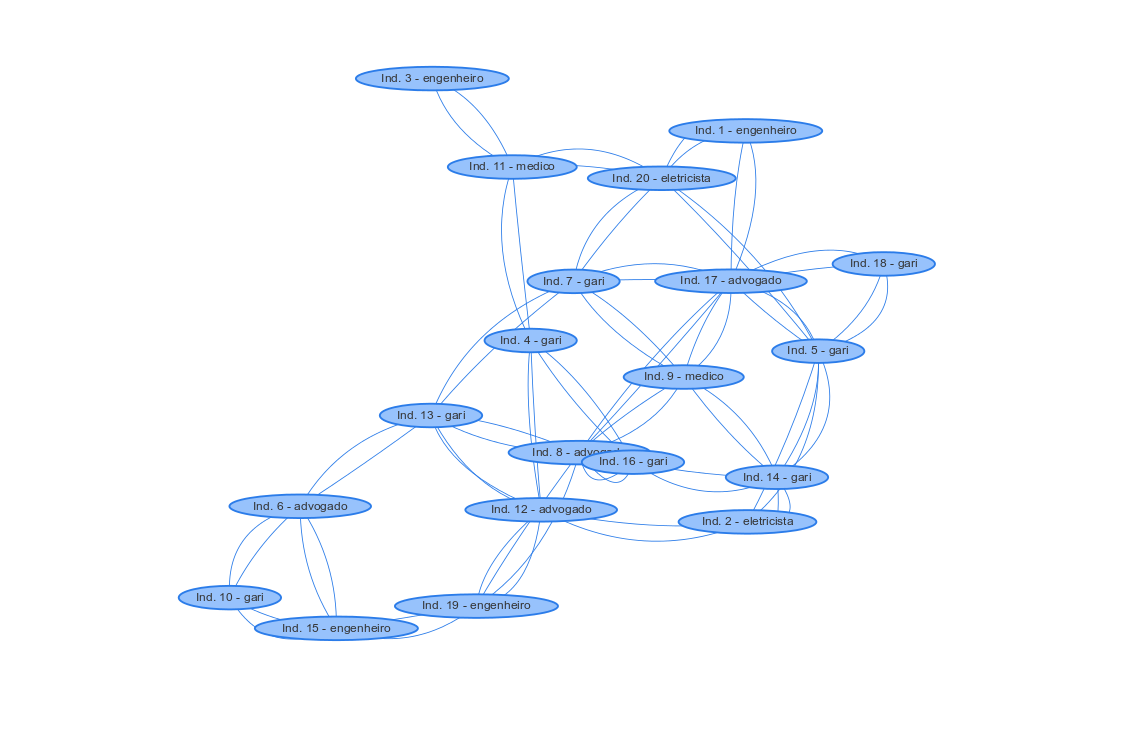
\includegraphics[scale=0.4]{./02-figuras/vis.png}
	\label{fig:patoB}
\end{figure*}

Após essa rede ter sido gerada, substituiu-se a geração aleatórias de redes sociais por essa rede gerada, para facilitar a simulação e consequentemente a validação dos resultados obtidos.

Tendo-se a rede social gerada (e consequentemente um grafo), desenvolveu-se a busca de prestadores de serviço à partir de um indivíduo, seus amigos e os amigos de seus amigos.

Para isso, implementou-se a função profissionais, que recebe como parâmetros g (rede social), individuo e profissão desejada. A função realiza uma busca de profundidade limitada ao segundo nível alcançável pelo indivíduo no grafo g e retorna todos os individuos alcançáveis até o segundo nível que atendem à profissão desejada.

A busca em profundidade limitada usa a mesma técnica da busca em profundidade, de utilizar-se uma pilha para visitação dos nodos, só que com a limitação do nível da busca, ela não permite que os nós abaixo do segundo nível sejam inseridos na pilha.

A \textbf{Figura \ref{fig:patoA}} mostra a implementação da função profissionais

\begin{figure*}
	\centering
	\caption{profissional - Função que realiza DLS até o nível 2 de um indivíduo da rede social e retorna indivíduos que prestam o serviço desejado} 
	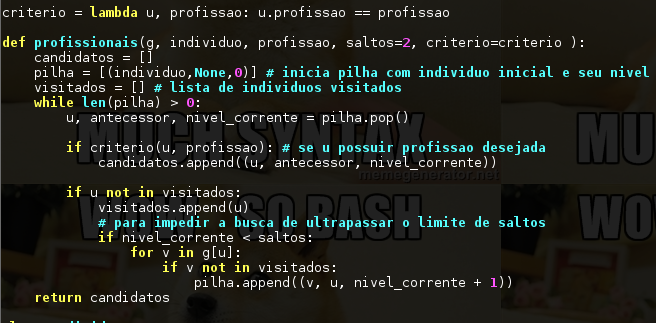
\includegraphics[scale=0.4]{./02-figuras/profissionais.png}
	\label{fig:patoA}
\end{figure*}
	% Arquivo a ser editado: contém a seção de “desenvolvimento” do artigo
% -----------------------------------------------------------------------------
%   Arquivo: ./01-texto/execucoes.tex
% -----------------------------------------------------------------------------

\section{Execuções}\label{sec:execucoes}    % edite para alterar o título da seção

Tendo-se implementado todas as classes, funções e estruturas necessárias para a simulação da rede social, executaram-se alguns testes para averiguar o correto funcionamento da busca em produndidade limitada.

A execução do programa é feita pelo seguinte comando:

{\tiny python -i profissionais.py}

Então, o python executa a geração da rede social e um terminal python é disponibilizado para a execução das simulações.

Todos os indivíduos encontram-se na lista indivíduos e para acessar um individuo, é necessário buscá-lo nessa lista. Se o indivíduo a ser acessado for o segundo, deve-se acessar a posição 1 da lista de indivíduos. Exemplo: individuos[1].

Tomando ainda como exemplo o segundo indivíduo, pela visualização gerada na biblioteca vis constata-se que esse indivíduo é um eletricista que é amigo dos individuos: 5 - gari, 12 - advogado e 14 - gari. Partindo-se deste indivíduo com o objetivo de encontrar um profissional que seja engenheiro, a execução da função profissionais deve retornar somente um profissional candidato: o indivíduo 19 - engenheiro que é amigo do individuo 12 - advogado, amigo do 1 - eletricista.

E a execução da função profissionais retornou exatamente só esse indivíduo candidato a dois níveis de distância, informando ainda o amigo que eles tem em comum - indivíduo 12, advogado.

Mais 10 execuções foram realizadas selecionando-se indivíduos aleatóriamente na rede social assim como suas profissões todos os resultados são validados na visualização da rede social.

A \textbf{Figura 7} mostra as execuções

\begin{figure*}
        \centering
        \caption{10 Execuções, validadas a olho nu com a visualização gráfica da rede social}
        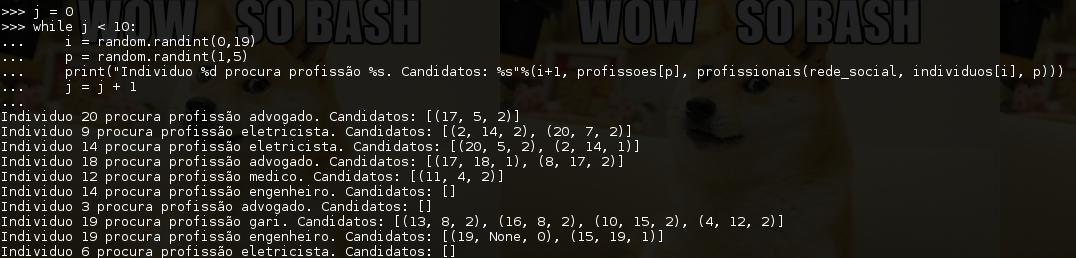
\includegraphics[scale=0.4]{./02-figuras/execucoes.png}
        \label{fig:execucoes}
\end{figure*}
	% Arquivo a ser editado: contém a seção de “execucoes” do artigo
% -----------------------------------------------------------------------------
%   Arquivo: ./01-texto/conclusao.tex
% -----------------------------------------------------------------------------


\section{Conclusão}\label{sec:conclusao}

A implementação da busca em profundidade limitada mostrou-se ser adequada para a implementação da idéia proposta pelo professor Dr. Fábio Rocha da Silva.
Apesar dele não ter mencionado as restrições de contactar somente amigos ou amigos de amigos para prestação de serviços, os autores deste artigo acharam por bem implementar dessa forma, de maneira a tentar aproximar a realidade do ambiente virtual da maneira mais fidedigna possível no que diz a questão de confiança. É bem mais fácil confiar em amigos ou amigos de amigos do que em completos desconhecidos. Porém, com o grande avanço das redes sociais, hoje tornou-se comum adicionar pessoas que não possuem forte vinculo de amizade, pessoas que são apenas conhecidas. Por isso, na questão de confiança, essa parte pode ficar um pouco comprometida para usuários que apresentam a característica de ter amigos além do seu círculo de amizade íntimo cotidiano em suas redes sociais. Porém, esse trabalho abre um caminho para uma área não muito bem explorada até o momento e que pode apresentar grande potencial rentável.

As seguintes funcionalidades podem ser aprimoradas a este trabalho para uma maior agregação de valor:

- Distinguir conhecidos de amigos
- Implementar um sistema de classificação de prestadores de serviço, assim como de clientes
- Implementar um sistema de pagamentos entre prestadores e clientes que permita realizar seguro para prestação de serviços, bem como a fração de pagamentos em etapas concluídas do serviço
- Implementar um sistema que permita a associação em grupos, tanto por prestadores de serviço quanto por clientes, para facilitar ambas as partes
		% Arquivo a ser editado: contém a seção de “conclusão” do artigo

	% Caso necessário, qualquer dos arquivos anteriores podem ser copiados e renomeados de modo a criar novas seções


%   Insere elementos pós-textuais

% -----------------------------------------------------------------------------
%   Arquivo: ./01-texto/agradecimentos.tex
% -----------------------------------------------------------------------------


\chapter{Agradecimentos}\label{sec:agradecimentos}

A Deus nosso senhor, que nos concedeu o dom da vida e tudo mais, para realizar este trabalho!

A nossa alma mater, O CEFET que nos proporciona a infraestrutura adequada para caminhar o caminho!

A nossos professores, que são os gigantes que colocam-nos sobre seus ombros para enxergarmos mais longe!

A nossas famílias, que são a base, o nosso porto seguro e nosso ponto de equilíbrio, a nossa fuga da insanidade!

E a todos os nossos amigos e colegas, companheiros dessa caminhada!

Louvado Seja Nosso Senhor Jesus Cristo!
Para Sempre Seja Louvado!
	% Arquivo a ser editado: contém os “agradecimentos” a pessoas e/ou instituições que apoiaram a realização do trabalho
			% Não se pode esquecer de agradecer apropriadamente às instituições de fomento à pesquisa
% -----------------------------------------------------------------------------
%   Arquivo: ./01-texto/abstract.tex
% -----------------------------------------------------------------------------


\chapter{Abstract}\label{sec:abstract}
Finding service providers can be an arduous task. This paper proposes the use of social networks to facilitate this process by selecting professionals from friends or at most friends of friends of a user in order to bring the traditions present in the real world ( to ask for professional indications to friends to avoid trust issues ) to the extent of virtual friendships.

To find such providers, a social network is mapped into a graph and a level 2 depth limited search is applied from a person p to his friends and friends of his friends to achieve the expected results: a list of individuals who provide a desired service where these individuals are direct user's friends or the user's friends of friends.
% -----------------------------------------------------------------------------
%   Edite o texto acima. Mantenha o limite de 200 palavras, bem como a formatação em parágrafo único.
% -----------------------------------------------------------------------------
			% Arquivo a ser editado: contém o “abstract” em inglês
% -----------------------------------------------------------------------------
%   Arquivo: ./04-referencias/referencias.tex
% -----------------------------------------------------------------------------



% -----------------------------------------------------------------------------
%   Carrega o arquivo “myRefs.bib” e extrai automaticamente as referências citadas
% -----------------------------------------------------------------------------

\bibliography{./04-referencias/myRefs.bib}{}
\bibliographystyle{abntex2-alf}		% Define o estilo ABNT para formatar a lista de referências  


% -----------------------------------------------------------------------------
%   Este arquivo não necessita de ser editado.
% -----------------------------------------------------------------------------
	% Arquivo não-editável: carrega o arquivo “myrefs.bib” (coloque-o no diretório raiz) e o formata conforme a ABNT

\end{document}
